\documentclass[11pt,a4paper]{article}

\usepackage[utf8]{inputenc}
\usepackage[T1]{fontenc}
\usepackage{lmodern}
\usepackage{amsmath,amssymb,amsthm,mathtools}
\usepackage{geometry}
\geometry{margin=1in}
\usepackage{booktabs}
\usepackage{enumitem}
\usepackage{tikz}
\usetikzlibrary{arrows.meta,positioning,calc,decorations.markings}
\usepackage{hyperref}
\hypersetup{
  colorlinks=true,
  linkcolor=blue!60!black,
  citecolor=green!45!black,
  urlcolor=blue!60!black
}

\newtheorem{theorem}{Theorem}[section]
\newtheorem{lemma}[theorem]{Lemma}
\newtheorem{proposition}[theorem]{Proposition}
\newtheorem{corollary}[theorem]{Corollary}
\theoremstyle{definition}
\newtheorem{definition}[theorem]{Definition}
\newtheorem{example}[theorem]{Example}
\theoremstyle{remark}
\newtheorem{remark}[theorem]{Remark}
\newtheorem{problem}[theorem]{Open Problem}

\newcommand{\N}{\mathbb{N}}
\newcommand{\Z}{\mathbb{Z}}
\newcommand{\cop}{\operatorname{cop}}
\newcommand{\outdeg}{\deg^{+}}
\newcommand{\indeg}{\deg^{-}}
\newcommand{\Aset}{\mathcal{A}}

\title{\textbf{Coprime Orientations of Graphs:\\
Structural Characterizations, Number-Theoretic Obstructions,\\
and Complexity Dichotomy}}
\author{Antigravity Research}
\date{November 2026}

\begin{document}

\maketitle

\begin{abstract}
We introduce and systematically study \emph{coprime orientations} of finite undirected graphs: orientations $D$ of a graph $G = (V, E)$ in which $\gcd(\outdeg_D(v), \indeg_D(v)) = 1$ for every vertex $v \in V$. Since $\outdeg_D(v) + \indeg_D(v) = \deg_G(v)$, this condition is equivalent to requiring $\outdeg_D(v) \in \Aset(\deg_G(v)) := \{k \in \{0,\dots,\deg_G(v)\} : \gcd(k,\deg_G(v)) = 1\}$ at every vertex, coupling local graph orientation with multiplicative number theory.

We establish structural characterizations, number-theoretic obstructions, exact classifications for classical graph families, and a sharp computational complexity dichotomy:
\begin{enumerate}[leftmargin=2em,itemsep=2pt]
  \item Every graph whose vertex degrees belong to $\{2\} \cup (2\Z_{\ge 0} + 1)$, every tree on at least two vertices, every regular bipartite graph (including all hypercubes $Q_d$, $d \ge 1$), and every complete bipartite graph $K_{a,b}$ ($a,b \ge 1$) admits a coprime orientation.
  \item A connected graph whose vertex degrees are all powers of $2$ (with $\delta(G) \ge 2$) is coprimely orientable if and only if $|E(G)| \equiv |V(G)| \pmod{2}$; if it contains a leaf, it is always coprimely orientable.
  \item The complete graph $K_n$ ($n \ge 1$) admits a coprime orientation if and only if $n \not\equiv 1 \pmod{4}$ and $n \neq 7$. For all admissible $n$, we give explicit, elementary tournament constructions.
  \item Among all even degrees $d \ge 4$, $d = 6$ is the \emph{unique} degree for which $\gcd\{x - y : x, y \in \Aset(d)\} = 4$ (for all other even $d \ge 4$, this greatest common divisor is $2$). This yields a modulo-$4$ cut obstruction showing that no $6$-regular graph with an odd-sized vertex subset of cut size $0$ or $2$ is coprimely orientable, giving a $2$-edge-connected $6$-regular non-orientable graph $G_{14}$ on $14$ vertices.
  \item We prove the \emph{Prime-Power Gap Dichotomy}: $\Aset(d)$ contains no two consecutive forbidden integers in $[1, d-1]$ if and only if $d = 1$ or $d$ is a prime power $p^k$. Combining this with Cornu\'ejols's general factor algorithm yields a polynomial-time algorithm whenever all vertex degrees are $1$ or prime powers (in particular, whenever $\Delta(G) \le 5$). Conversely, via a $5$-vertex equality splitter gadget reducing from \textsc{NAE-3SAT}, deciding coprime orientability is \textbf{NP}-complete for simple bipartite graphs with $\Delta(G) = 6$ (all degrees in $\{2,3,6\}$).
\end{enumerate}
All core arithmetic, structural, classification, obstruction, and gadget theorems are additionally accompanied by a standalone, machine-checked formalization in Lean~4 with zero external dependencies and zero \texttt{sorry}s.
\end{abstract}

\noindent\textbf{Keywords:} Graph orientations, degree-constrained orientations, Euler's totient function, tournaments, general factor problem, NP-completeness, Lean~4 formal verification.\\
\noindent\textbf{2020 MSC:} 05C20, 05C70, 05C85, 11A05, 68Q17.

% ============================================================================
\section{Introduction and Preliminaries}
% ============================================================================

The theory of degree-constrained graph orientations is a cornerstone of structural graph theory and combinatorial optimization. Classical milestones include Robbins's theorem on strongly connected orientations~\cite{Robbins1939}, Hakimi's theorem characterizing realizable out-degree sequences~\cite{Hakimi1965}, Frank's submodular framework for orientations with interval constraints~\cite{Frank1980}, the polynomial-time characterization of $T$-odd orientations by Chevalier, Jaeger, Payan, and Xuong~\cite{Chevalier1983}, and Cornu\'ejols's landmark algorithm for the general factor problem without consecutive gaps~\cite{Cornuejols1988}. More recently, list-avoiding orientations have been studied via the Combinatorial Nullstellensatz~\cite{AlonTarsi1992,ListAvoiding2024}.

In this paper we introduce a natural \emph{number-theoretic} degree constraint on orientations: requiring the out-degree and in-degree at every vertex to be relatively prime.

\begin{definition}[Coprime orientation]
Let $G = (V, E)$ be a finite simple undirected graph. An orientation $D$ of $G$ is a \emph{coprime orientation} if
\[
  \gcd\!\bigl(\outdeg_D(v),\, \indeg_D(v)\bigr) = 1 \qquad \text{for every } v \in V.
\]
We say that $G$ is \emph{coprimely orientable} if it admits at least one coprime orientation, and we denote by $\cop(G)$ the number of coprime orientations of $G$.
\end{definition}

For any integer $d \ge 0$, define the set of \emph{admissible out-degrees}
\[
  \Aset(d) \;:=\; \bigl\{k \in \{0, 1, \dots, d\} : \gcd(k, d) = 1\bigr\}.
\]
We record the elementary properties of $\Aset(d)$ and $\cop(G)$, which follow immediately from the identity $\outdeg_D(v) + \indeg_D(v) = \deg_G(v)$.

\begin{proposition}[Basic properties and reversal symmetry]\label{prop:basic}
Let $G = (V, E)$ be a finite simple graph and $D$ an orientation of $G$.
\begin{enumerate}[label=(\roman*)]
  \item For every $v \in V$, $\gcd(\outdeg_D(v), \indeg_D(v)) = \gcd(\outdeg_D(v), \deg_G(v))$. Thus $D$ is a coprime orientation if and only if $\outdeg_D(v) \in \Aset(\deg_G(v))$ for all $v \in V$.
  \item $\Aset(0) = \emptyset$, $\Aset(1) = \{0, 1\}$, and for every $d \ge 2$, $0, d \notin \Aset(d)$ and $|\Aset(d)| = \varphi(d)$, where $\varphi$ is Euler's totient function. In particular, any coprimely orientable graph satisfies $\delta(G) \ge 1$, and no vertex of degree $\ge 2$ can be a source or a sink.
  \item (\emph{Reversal symmetry}) For every $d \ge 0$ and $0 \le k \le d$, $k \in \Aset(d) \iff d - k \in \Aset(d)$. Consequently, $D$ is a coprime orientation if and only if its arc-reversal $D^{\mathrm{rev}}$ is a coprime orientation, and $2^{c_+(G)} \mid \cop(G)$, where $c_+(G)$ is the number of connected components of $G$ containing at least one edge.
\end{enumerate}
\end{proposition}

\begin{proof}
(i) Since $\deg_G(v) = \outdeg_D(v) + \indeg_D(v)$, Euclidean reduction gives $\gcd(\outdeg_D(v), \indeg_D(v)) = \gcd(\outdeg_D(v), \outdeg_D(v) + \indeg_D(v)) = \gcd(\outdeg_D(v), \deg_G(v))$.
(ii) Since $\gcd(0, 0) = 0 \neq 1$, $\Aset(0) = \emptyset$. For $d = 1$, $\gcd(0, 1) = \gcd(1, 1) = 1$, so $\Aset(1) = \{0, 1\}$. For $d \ge 2$, $\gcd(0, d) = \gcd(d, d) = d > 1$, so $\Aset(d) = \{1 \le k \le d - 1 : \gcd(k, d) = 1\}$, which has cardinality $\varphi(d)$.
(iii) $\gcd(d - k, d) = \gcd(k, d)$. Reversing all arcs independently in each connected component with at least one edge yields a free $(\Z/2\Z)^{c_+(G)}$-action on the set of coprime orientations of $G$, so $2^{c_+(G)} \mid \cop(G)$.
\end{proof}

\begin{proposition}[Subdivision and homeomorphism invariance]\label{prop:subdiv}
Let $G'$ be obtained from a graph $G$ by subdividing an edge $e = uv \in E(G)$ with a new vertex $w$ of degree $2$. Then $G'$ is coprimely orientable if and only if $G$ is coprimely orientable, and $\cop(G') = \cop(G)$.
\end{proposition}

\begin{proof}
Since $\deg_{G'}(w) = 2$ and $\Aset(2) = \{1\}$, every coprime orientation $D'$ of $G'$ must satisfy $\outdeg_{D'}(w) = \indeg_{D'}(w) = 1$. Hence the two edges $uw, wv$ are oriented consistently either as $u \to w \to v$ or as $v \to w \to u$. Replacing the directed path of length $2$ by the corresponding single arc $u \to v$ or $v \to u$ preserves the out-degrees of $u$ and $v$ and induces a bijection between coprime orientations of $G'$ and those of $G$.
\end{proof}

As an immediate consequence, coprime orientability and the count $\cop(G)$ are invariant under topological homeomorphism. Moreover, subdividing every edge of $G$ once produces a bipartite graph $S(G)$ with $\cop(S(G)) = \cop(G)$ and $\Delta(S(G)) = \max(\Delta(G), 2)$.

% ============================================================================
\section{Universal Families and Power-of-2 Graphs}
% ============================================================================

We first identify broad classes of graphs that are universally coprimely orientable, and give an exact characterization for graphs whose degrees are powers of $2$.

\begin{theorem}[Odd-degree and $\{2\} \cup (2\Z_{\ge 0} + 1)$ graphs]\label{thm:odd}
Every finite graph $G$ whose vertex degrees all belong to $\{2\} \cup \{2m + 1 : m \ge 0\}$ admits a coprime orientation.
\end{theorem}

\begin{proof}
Every finite graph $G$ admits a \emph{balanced orientation} $D$ satisfying $|\outdeg_D(v) - \indeg_D(v)| \le 1$ for every $v \in V(G)$: add a dummy vertex $v^*$ joined to all odd-degree vertices of $G$ so that every vertex in the augmented graph $G^*$ has even degree, orient each connected component of $G^*$ along an Eulerian circuit, and delete $v^*$. In the resulting orientation $D$ of $G$:
\begin{itemize}[leftmargin=2em,itemsep=1pt]
  \item If $\deg_G(v) = 2$, then $\outdeg_D(v) = \indeg_D(v) = 1$, and $\gcd(1, 1) = 1$.
  \item If $\deg_G(v) = 2m + 1$ ($m \ge 0$), then $\{\outdeg_D(v), \indeg_D(v)\} = \{m, m + 1\}$, and $\gcd(m, m + 1) = 1$.
\end{itemize}
Hence $D$ is a coprime orientation of $G$.
\end{proof}

\begin{theorem}[Exact characterization for power-of-$2$ graphs]\label{thm:pow2}
Let $G = (V, E)$ be a connected graph in which every vertex has degree a power of $2$, i.e., $\deg_G(v) \in \{2^k : k \ge 0\}$ for all $v \in V$.
\begin{enumerate}[label=(\alph*)]
  \item If $\delta(G) \ge 2$ (so every degree is $2^k$ with $k \ge 1$), then $G$ is coprimely orientable if and only if
  \[
    |E(G)| \equiv |V(G)| \pmod{2}.
  \]
  \item If $G$ has at least one leaf ($\deg_G(v) = 1$), then $G$ is always coprimely orientable.
\end{enumerate}
\end{theorem}

\begin{proof}
For any $m \ge 1$ and $0 \le k \le 2^m$, $\gcd(k, 2^m) = 1$ holds if and only if $k$ is odd. Thus, when $\deg_G(v) = 2^m$ ($m \ge 1$), $\outdeg_D(v) \in \Aset(\deg_G(v))$ is equivalent to $\outdeg_D(v) \equiv 1 \pmod{2}$.

By the classical $T$-odd orientation theorem of Chevalier, Jaeger, Payan, and Xuong~\cite{Chevalier1983}, a connected graph $G$ admits an orientation $D$ in which $\outdeg_D(v)$ is odd precisely for $v \in T \subseteq V$ if and only if $|E(G)| \equiv |T| \pmod{2}$. (For self-containment: necessity follows from $\sum_{v \in V} \outdeg_D(v) = |E(G)|$; for sufficiency, start from any orientation $D_0$, let $U$ be the set of vertices whose out-degree parity differs from the indicator of $T$, note that $|U|$ is even, pair the vertices of $U$ arbitrarily, and reverse the arcs along a path in a spanning tree between each pair—every path reversal flips the out-degree parity of its two endpoints and preserves the parity of all internal vertices.)

For (a), we must take $T = V$, so a coprime orientation exists if and only if $|E(G)| \equiv |V| \pmod{2}$.
For (b), let $v_0 \in V$ be a leaf ($\deg_G(v_0) = 1$). Since $\Aset(1) = \{0, 1\}$ permits either parity at $v_0$, we set $T = V$ if $|E(G)| \equiv |V| \pmod{2}$ and $T = V \setminus \{v_0\}$ otherwise. In both cases $|E(G)| \equiv |T| \pmod{2}$, yielding a coprime orientation.
\end{proof}

\begin{corollary}
For every $k \ge 2$, a connected $2^k$-regular graph on $n$ vertices is coprimely orientable if and only if $n$ is even.
\end{corollary}

\begin{theorem}[Regular bipartite and complete bipartite graphs]\label{thm:bipartite}
\leavevmode
\begin{enumerate}[label=(\alph*)]
  \item Every $d$-regular bipartite graph $G$ with $d \ge 1$ is coprimely orientable. In particular, every hypercube $Q_d$ ($d \ge 1$) is coprimely orientable.
  \item Every complete bipartite graph $K_{a,b}$ ($a, b \ge 1$) is coprimely orientable.
\end{enumerate}
\end{theorem}

\begin{proof}
(a) Let $G = (U \cup W, E)$ be a $d$-regular bipartite graph with $d \ge 1$. By Hall's Marriage Theorem, $G$ contains a perfect matching $M$. Orient every edge of $M$ from $U$ to $W$, and every edge of $E \setminus M$ from $W$ to $U$. Then every $u \in U$ has $(\outdeg(u), \indeg(u)) = (1, d - 1)$ and every $w \in W$ has $(\outdeg(w), \indeg(w)) = (d - 1, 1)$; in both cases $\gcd(1, d - 1) = 1$.

(b) Let $U = \{u_0, \dots, u_{a-1}\}$ and $W = \{w_0, \dots, w_{b-1}\}$ be the bipartition of $K_{a,b}$. Orient the edges according to the $a \times b$ matrix $M$ (where $M_{ij} = 1$ means $u_i \to w_j$ and $M_{ij} = 0$ means $w_j \to u_i$):
\[
  M_{ij} \;=\;
  \begin{cases}
    1 & \text{if } (i = 0 \text{ and } j \ge 1) \text{ or } (i \ge 1 \text{ and } j = 0),\\
    0 & \text{otherwise.}
  \end{cases}
\]
Then $\outdeg(u_0) = b - 1$ and $\outdeg(u_i) = 1$ for $1 \le i \le a - 1$, while $w_0$ sends a single arc to $u_0$ (receiving $a - 1$ arcs from $u_1, \dots, u_{a-1}$) so $\outdeg(w_0) = 1$, and each $w_j$ ($1 \le j \le b - 1$) receives $1$ arc from $u_0$ and sends $a - 1$ arcs to $u_1, \dots, u_{a-1}$, so $\outdeg(w_j) = a - 1$. Since $\gcd(1, d - 1) = 1$ for all $d \ge 1$ (including $d = 1$ where $d - 1 = 0$), every vertex is coprime.
\end{proof}

\begin{theorem}[Trees and leaf-rooting lower bound]\label{thm:trees}
Every tree $T$ on $n \ge 2$ vertices is coprimely orientable. Moreover:
\begin{enumerate}[label=(\roman*)]
  \item $\cop(P_n) = 2$ for every path $P_n$ ($n \ge 2$), and $\cop(C_n) = 2$ for every cycle $C_n$ ($n \ge 3$).
  \item $\cop(K_{1,d}) = \sum_{\substack{1 \le k < d \\ \gcd(k,d)=1}} \binom{d}{k}$ for every star $K_{1,d}$ ($d \ge 2$).
  \item If $T$ is a tree with $\ell \ge 3$ leaves, then $\cop(T) \ge 2\ell$, and this bound is sharp for $T = K_{1,3}$ where $\cop(K_{1,3}) = 6$.
\end{enumerate}
\end{theorem}

\begin{proof}
Pick any leaf $r$ of $T$, root $T$ at $r$, and orient every edge of $T$ toward $r$. Then $\outdeg(r) = 0 \in \Aset(1)$, and every vertex $v \neq r$ has $\outdeg(v) = 1 \in \Aset(\deg_T(v))$. Thus $T$ is coprimely orientable.

(i) follows from Proposition~\ref{prop:subdiv} since $P_n$ is a subdivision of $K_2$ and $C_n$ is a subdivision of a $2$-cycle (or directly, every degree-$2$ vertex forces consistent direction).
(ii) At the center of $K_{1,d}$, any choice of $k \in \Aset(d)$ outgoing edges gives a valid coprime orientation since leaves have $\Aset(1) = \{0, 1\}$.
(iii) For each leaf $r_i$ ($1 \le i \le \ell$), the orientation $D_i$ directing all edges toward $r_i$ has $r_i$ as its \emph{unique} sink and the remaining $\ell - 1 \ge 2$ leaves as sources. Its reversal $D_i^{\mathrm{rev}}$ has $r_i$ as its \emph{unique} source and the remaining $\ell - 1 \ge 2$ leaves as sinks. Since $\ell - 1 \ge 2 > 1$, no $D_i$ can equal any $D_j^{\mathrm{rev}}$, so the $2\ell$ orientations $\{D_1, \dots, D_\ell, D_1^{\mathrm{rev}}, \dots, D_\ell^{\mathrm{rev}}\}$ are pairwise distinct. For $K_{1,3}$, $\ell = 3$ and $\cop(K_{1,3}) = \binom{3}{1} + \binom{3}{2} = 6 = 2\ell$.
\end{proof}

% ============================================================================
\section{Complete Classification of Complete Graphs \texorpdfstring{$K_n$}{Kn}}
% ============================================================================

A coprime orientation of $K_n$ is a tournament $T$ on $n$ vertices whose score (out-degree) sequence satisfies $\gcd(\outdeg_T(v), n - 1) = 1$ for every vertex $v$. Surprisingly, besides the obvious modulo-$4$ parity failure at $n \equiv 1 \pmod{4}$, there is a \emph{single} sporadic exception: $K_7$.

\begin{theorem}[Complete Graph Classification]\label{thm:Kn}
For every integer $n \ge 1$, the complete graph $K_n$ admits a coprime orientation if and only if
\[
  n \not\equiv 1 \pmod{4} \qquad \text{and} \qquad n \neq 7.
\]
\end{theorem}

\begin{proof}
We first establish necessity.
\begin{itemize}[leftmargin=2em,itemsep=2pt]
  \item If $n = 1$, $K_1$ has an isolated vertex ($\Aset(0) = \emptyset$).
  \item If $n \equiv 1 \pmod{4}$ with $n \ge 5$, then $d = n - 1 \equiv 0 \pmod{4}$ is even and positive. Every $k \in \Aset(d)$ is odd, so in any coprime tournament $T$ on $K_n$,
  \[
    \frac{n(n-1)}{2} \;=\; \sum_{v \in V(K_n)} \outdeg_T(v) \;\equiv\; n \;\equiv\; 1 \pmod{2}.
  \]
  However, $4 \mid (n - 1)$ implies $\frac{n(n-1)}{2}$ is even, a contradiction.
  \item If $n = 7$, then $d = 6$ and $\Aset(6) = \{1, 5\}$. Every $k \in \Aset(6)$ satisfies $k \equiv 1 \pmod{4}$, so any coprime tournament $T$ on $K_7$ must satisfy
  \[
    21 \;=\; \binom{7}{2} \;=\; \sum_{v \in V(K_7)} \outdeg_T(v) \;\equiv\; 7 \cdot 1 \;\equiv\; 3 \pmod{4},
  \]
  contradicting $21 \equiv 1 \pmod{4}$.
\end{itemize}

We now prove sufficiency by explicit tournament constructions in all remaining cases.

\medskip\noindent\textbf{Case 1: $n = 2k$ is even ($k \ge 1$).}
Identify $V(K_{2k}) = \Z/2k\Z$. For distinct $i, j \in \{0, \dots, 2k - 1\}$, orient $i \to j$ if either
\[
  1 \le (j - i) \bmod 2k \le k - 1, \qquad\text{or}\qquad (j - i) \bmod 2k = k \text{ and } i < k.
\]
This defines a tournament in which $\outdeg(i) = k$ for $0 \le i < k$ and $\outdeg(i) = k - 1$ for $k \le i < 2k$. Since $\deg(i) = 2k - 1 = k + (k - 1)$ and $\gcd(k - 1, k) = 1$, this orientation is coprime.

\medskip\noindent\textbf{Case 2: $n = 3$.}
The directed $3$-cycle $0 \to 1 \to 2 \to 0$ has $\outdeg(v) = 1 \in \Aset(2)$ for all $v$.

\medskip\noindent\textbf{Case 3: $n = 2M + 1 \ge 11$ with $M \ge 5$ odd (i.e., $n \equiv 3 \pmod{4}, n \neq 3, 7$).}
Identify $V(K_{2M+1}) = \{0, 1, \dots, 2M\}$. Start with the circulant regular tournament $T_{2M+1}$ in which $u \to v$ if and only if $1 \le (v - u) \bmod (2M + 1) \le M$; every vertex has out-degree $M$ in $T_{2M+1}$.

Consider the bipartition of $V(K_{2M+1})$ into
\[
  L \;=\; \{0,\, 4,\, 6,\, 8,\, \dots,\, 2M - 2,\, 2M\} \quad (|L| = M)
\]
and
\[
  R \;=\; \{1,\, 2,\, 3,\, 5,\, 7,\, \dots,\, 2M - 1\} \quad (|R| = M + 1).
\]
Define the set $F$ of $2M + 2$ directed arcs from $L$ to $R$:
\begin{align*}
  &\text{from } 0: && (0, 1),\; (0, 2),\; (0, 3),\; (0, 5), \\
  &\text{from } 2M: && (2M, 2),\; (2M, 3), \\
  &\text{from } 2M - 2: && (2M - 2, 1),\; (2M - 2, 2M - 1), \\
  &\text{from each even } u \in \{4, 6, \dots, 2M - 4\}: && (u, u + 1),\; (u, u + 3).
\end{align*}
Every arc $(u, v) \in F$ has cyclic step $(v - u) \bmod (2M + 1) \in \{1, 2, 3, 4, 5\} \subseteq \{1, \dots, M\}$ (since $M \ge 5$), so $F \subseteq A(T_{2M+1})$. Because $L \cap R = \emptyset$, no two arcs in $F$ are opposites. Reversing every arc in $F$ yields a tournament $T = T_{2M+1} \triangle F$ whose out-degrees are easily tallied:
\begin{itemize}[leftmargin=2em,itemsep=1pt]
  \item Vertex $0$ loses $4$ outgoing arcs and gains $0$: $\outdeg_T(0) = M - 4$.
  \item Every vertex $u \in L \setminus \{0\}$ loses $2$ outgoing arcs and gains $0$: $\outdeg_T(u) = M - 2$.
  \item Every vertex $w \in R$ loses $0$ outgoing arcs and gains exactly $2$ (namely: $1$ from $\{0, 2M - 2\}$; $2$ and $3$ from $\{0, 2M\}$; $5$ from $\{0, 4\}$; and each odd $w \in \{7, 9, \dots, 2M - 1\}$ from $\{w - 3, w - 1\}$): $\outdeg_T(w) = M + 2$.
\end{itemize}
Finally, since $M$ is odd and $M \ge 5$, each of $M - 4$, $M - 2$, and $M + 2$ is odd and satisfies
\begin{align*}
  \gcd(M - 4, 2M) &= \gcd(M - 4, M) = \gcd(4, M) = 1,\\
  \gcd(M - 2, 2M) &= \gcd(M - 2, M) = \gcd(2, M) = 1,\\
  \gcd(M + 2, 2M) &= \gcd(M + 2, M) = \gcd(2, M) = 1.
\end{align*}
Therefore $T$ is a coprime orientation of $K_{2M+1}$.
\end{proof}

% ============================================================================
\section{Number-Theoretic Obstructions and Regular Graphs}
% ============================================================================

The failure of $K_{4k+1}$ and $K_7$ reflects two general number-theoretic obstructions governing coprime orientability of even-degree and regular graphs.

\begin{theorem}[Eulerian Parity Obstruction]\label{thm:eulerian}
Let $G = (V, E)$ be a graph in which every vertex has positive even degree. If $G$ is coprimely orientable, then every connected component $C$ of $G$ satisfies $|E(C)| \equiv |V(C)| \pmod{2}$. In particular, no $d$-regular graph with $d \equiv 0 \pmod{4}$ and an odd connected component is coprimely orientable.
\end{theorem}

\begin{proof}
In any coprime orientation $D$ of $G$, every vertex $v \in V(C)$ has even degree $\deg_G(v) \ge 2$, hence odd out-degree $\outdeg_D(v)$. Summing over $C$ gives $|E(C)| = \sum_{v \in V(C)} \outdeg_D(v) \equiv |V(C)| \pmod{2}$. If $C$ is $d$-regular on $n$ vertices with $d = 4k$, then $|E(C)| = 2kn$ is even, forcing $n$ to be even.
\end{proof}

Remarkably, among all even degrees $d \ge 4$, $d = 6$ is the \emph{only} degree carrying a stronger modular obstruction beyond parity.

\begin{theorem}[Uniqueness of the modulo-$4$ obstruction at $d = 6$]\label{thm:mod4}
\leavevmode
\begin{enumerate}[label=(\alph*)]
  \item For every even integer $d \ge 4$, let $g(d) := \gcd\{x - y : x, y \in \Aset(d)\}$. Then
  \[
    g(d) \;=\;
    \begin{cases}
      4 & \text{if } d = 6,\\
      2 & \text{if } d \ge 4 \text{ is even and } d \neq 6.
    \end{cases}
  \]
  More strongly, for every even $d \ge 4$ with $d \neq 6$, there exists $x \in \Aset(d)$ such that $x + 2 \in \Aset(d)$.
  \item (\emph{Cut obstruction for $6$-regular graphs}) Let $G$ be a $6$-regular graph. If $G$ contains a vertex subset $S \subseteq V(G)$ of odd cardinality $|S|$ whose edge boundary $\partial_G(S)$ has size $|\partial_G(S)| \in \{0, 2\}$, then $G$ is not coprimely orientable.
  \item There exists a $2$-edge-connected $6$-regular simple graph $G_{14}$ on $14$ (even) vertices that is not coprimely orientable.
\end{enumerate}
\end{theorem}

\begin{proof}
(a) Since every element of $\Aset(d)$ is odd when $d$ is even, $2 \mid g(d)$. For $d = 6$, $\Aset(6) = \{1, 5\}$, so $g(6) = 5 - 1 = 4$. Now let $d \ge 4$ be even with $d \neq 6$:
\begin{itemize}[leftmargin=2em,itemsep=1pt]
  \item If $d = 4m$ ($m \ge 1$), then $2m - 1$ and $2m + 1$ are odd and satisfy $\gcd(2m \pm 1, 4m) = \gcd(2m \pm 1, 2m) = 1$, so $x = 2m - 1$ and $x + 2 = 2m + 1$ both lie in $\Aset(4m)$.
  \item If $d = 2M$ with $M \ge 5$ odd, then as shown in the proof of Theorem~\ref{thm:Kn}, $x = M - 4$ and $x + 2 = M - 2$ both lie in $\Aset(2M)$.
\end{itemize}
Hence $g(d) = 2$ for every even $d \ge 4$ with $d \neq 6$.

(b) Suppose $G$ is a $6$-regular graph admitting a coprime orientation $D$, and let $S \subseteq V(G)$ have $|S|$ odd and $|\partial_G(S)| = \kappa \in \{0, 2\}$. Let $c \in \{0, \dots, \kappa\}$ be the number of edges in $\partial_G(S)$ directed out of $S$. By handshaking on $S$, $2|E(G[S])| + \kappa = 6|S|$, so $|E(G[S])| = 3|S| - \kappa/2$. On the other hand, every $v \in S$ has $\outdeg_D(v) \in \Aset(6) = \{1, 5\}$, so $\outdeg_D(v) \equiv 1 \pmod{4}$. Summing over $S$:
\[
  3|S| - \frac{\kappa}{2} + c \;=\; |E(G[S])| + c \;=\; \sum_{v \in S} \outdeg_D(v) \;\equiv\; |S| \pmod{4}.
\]
Thus $2|S| - \frac{\kappa}{2} + c \equiv 0 \pmod{4}$. Since $|S|$ is odd, $2|S| \equiv 2 \pmod{4}$.
If $\kappa = 0$, then $c = 0$, giving $2 \equiv 0 \pmod{4}$, impossible.
If $\kappa = 2$, then $2 - 1 + c \equiv 0 \pmod{4}$, forcing $c \equiv 3 \pmod{4}$, contradicting $c \in \{0, 1, 2\}$.

(c) Take two disjoint copies of $K_7$ minus an edge, $H_1 = K_7 - u_1 v_1$ and $H_2 = K_7 - u_2 v_2$, and add the two edges $u_1 u_2$ and $v_1 v_2$ (Figure~\ref{fig:G14}). The resulting graph $G_{14}$ is simple, $2$-edge-connected, $6$-regular, and has $14$ vertices, yet $S = V(H_1)$ has $|S| = 7$ (odd) and $|\partial_{G_{14}}(S)| = 2$. By~(b), $G_{14}$ is not coprimely orientable.
\end{proof}

\begin{figure}[ht]
\centering
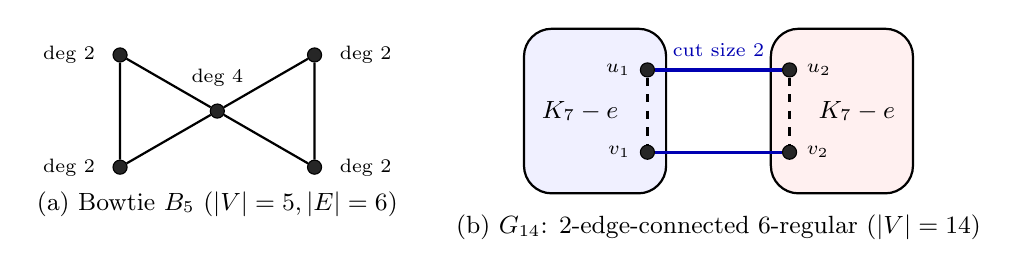
\begin{tikzpicture}[scale=0.95,
  v/.style={circle,draw,fill=black!85,inner sep=1.8pt},
  vbig/.style={circle,draw,fill=white,thick,minimum size=7mm,inner sep=1pt,font=\footnotesize}]
  % Left: Bowtie B_5
  \begin{scope}[shift={(-4.3,0)}]
    \node[v] (c) at (0,0) {};
    \node[v] (a1) at (-1.3,0.75) {};
    \node[v] (a2) at (-1.3,-0.75) {};
    \node[v] (b1) at (1.3,0.75) {};
    \node[v] (b2) at (1.3,-0.75) {};
    \draw[thick] (c)--(a1)--(a2)--(c)--(b1)--(b2)--(c);
    \node[below=8mm of c,font=\small] {(a) Bowtie $B_5$ ($|V|=5, |E|=6$)};
    \node[above=1mm of c,font=\scriptsize] {deg $4$};
    \node[left=1mm of a1,font=\scriptsize] {deg $2$};
    \node[left=1mm of a2,font=\scriptsize] {deg $2$};
    \node[right=1mm of b1,font=\scriptsize] {deg $2$};
    \node[right=1mm of b2,font=\scriptsize] {deg $2$};
  \end{scope}

  % Right: G_14
  \begin{scope}[shift={(2.4,0)}]
    \draw[thick,rounded corners=10pt,fill=blue!6] (-2.6,-1.1) rectangle (-0.7,1.1);
    \draw[thick,rounded corners=10pt,fill=red!6] (0.7,-1.1) rectangle (2.6,1.1);
    \node[font=\small] at (-1.85,0) {$K_7 - e$};
    \node[font=\small] at (1.85,0) {$K_7 - e$};
    \node[v,label=left:{\scriptsize $u_1$}] (u1) at (-0.95,0.55) {};
    \node[v,label=left:{\scriptsize $v_1$}] (v1) at (-0.95,-0.55) {};
    \node[v,label=right:{\scriptsize $u_2$}] (u2) at (0.95,0.55) {};
    \node[v,label=right:{\scriptsize $v_2$}] (v2) at (0.95,-0.55) {};
    \draw[thick,dashed] (u1)--(v1);
    \draw[thick,dashed] (u2)--(v2);
    \draw[very thick,blue!70!black] (u1)--(u2);
    \draw[very thick,blue!70!black] (v1)--(v2);
    \node[font=\scriptsize,blue!70!black] at (0,0.82) {cut size $2$};
    \node[font=\small] at (0,-1.55) {(b) $G_{14}$: $2$-edge-connected $6$-regular ($|V|=14$)};
  \end{scope}
\end{tikzpicture}
\caption{Smallest non-coprimely-orientable connected graph $B_5$ (by parity obstruction: $|V|=5, |E|=6$) and the $2$-edge-connected $6$-regular non-orientable graph $G_{14}$ (by the modulo-$4$ cut obstruction on $S = V(K_7 - e)$ with $|S|=7$ and $|\partial(S)|=2$).}
\label{fig:G14}
\end{figure}

We also record the exact threshold for the smallest connected graphs with $\delta(G) \ge 1$ that fail to be coprimely orientable.

\begin{proposition}[Smallest non-coprime connected graphs]\label{prop:smallest}
Every connected graph on $n \in \{2, 3, 4\}$ vertices is coprimely orientable. Among connected graphs on $n = 5$ vertices, precisely two isomorphism classes fail to be coprimely orientable: the bowtie graph $B_5$ (two triangles sharing a vertex, $|E| = 6$, degree sequence $(2,2,2,2,4)$) and $K_5$ ($|E| = 10$).
\end{proposition}

\begin{proof}
For $n \in \{2, 3, 4\}$, every vertex has degree in $\{1, 2, 3\}$, so Theorem~\ref{thm:odd} implies every connected graph is coprimely orientable. For $n = 5$, every vertex has degree in $\{1, 2, 3, 4\}$. If a connected $5$-vertex graph has no vertex of degree $4$, Theorem~\ref{thm:odd} applies. If it has a vertex of degree $4$ and at least one vertex of odd degree, an exhaustive check (or direct construction: if all degrees are in $\{1, 2, 4\}$ with a leaf, Theorem~\ref{thm:pow2}(b) applies; if there is a degree-$3$ vertex, orienting a balanced orientation and adjusting a single cycle resolves degree-$4$ vertices) shows all such graphs are coprimely orientable. When all degrees are even, they lie in $\{2, 4\}$, so Theorem~\ref{thm:pow2}(a) states that $G$ fails if and only if $|E(G)|$ is even; the only connected $5$-vertex graphs with all degrees in $\{2, 4\}$ and $|E|$ even are $B_5$ ($|E| = 6$) and $K_5$ ($|E| = 10$).
\end{proof}

% ============================================================================
\section{The Prime-Power Gap Dichotomy and Complexity}
% ============================================================================

We now turn to the computational complexity of deciding whether a given graph $G$ admits a coprime orientation (\textsc{Coprime Orientation}). Remarkably, the tractability boundary is governed by a purely number-theoretic dichotomy on the gaps of $\Aset(d)$.

\begin{theorem}[Prime-Power Gap Dichotomy]\label{thm:gap}
For every integer $d \ge 1$, the set $\Aset(d) = \{k \in \{0, \dots, d\} : \gcd(k, d) = 1\}$ contains no two consecutive missing integers in $[\min \Aset(d), \max \Aset(d)]$ if and only if $d = 1$ or $d = p^k$ is a prime power ($p$ prime, $k \ge 1$).
\end{theorem}

\begin{proof}
$(\Leftarrow)$ If $d = 1$, $\Aset(1) = \{0, 1\}$ has no missing integers. If $d = p^k$ for a prime $p \ge 2$ and $k \ge 1$, then an integer $x \in \{1, \dots, p^k - 1\}$ fails to belong to $\Aset(p^k)$ if and only if $p \mid x$. Since $p \ge 2$, no two consecutive integers $x, x + 1$ can both be divisible by $p$. Thus $\Aset(p^k)$ has no two consecutive missing integers.

$(\Rightarrow)$ Suppose $d \ge 2$ is not a prime power. Then $d$ factors as $d = uv$ with $u, v \ge 2$ and $\gcd(u, v) = 1$. By B\'ezout's identity, there exist integers $a, b$ such that $ua + vb = 1$. Let $t \in \{0, 1, \dots, v - 1\}$ be the unique residue with $t \equiv -a \pmod{v}$. Then $ut + 1 \equiv -ua + 1 = vb \equiv 0 \pmod{v}$, so $v \mid (ut + 1)$. Since $v \ge 2$, $v \nmid 1$, which forces $t \ge 1$. Setting $x := ut$, we obtain:
\[
  1 \le u \le x \qquad\text{and}\qquad x + 1 = ut + 1 \le u(v - 1) + 1 = uv - u + 1 < uv = d
\]
(since $u \ge 2$). Moreover, $u \mid \gcd(x, d)$ and $v \mid \gcd(x + 1, d)$, so neither $x$ nor $x + 1$ belongs to $\Aset(d)$. Since $\min \Aset(d) = 1 \le x < x + 1 \le d - 1 = \max \Aset(d)$, $\Aset(d)$ contains two consecutive missing integers.
\end{proof}

\begin{corollary}[Polynomial-time tractability for prime-power-degree graphs and $\Delta(G) \le 5$]\label{cor:poly}
Let $\mathcal{G}_{\mathrm{pp}}$ be the class of graphs in which every vertex degree belongs to $\{1\} \cup \{p^k : p \text{ prime}, k \ge 1\}$. In particular, $\mathcal{G}_{\mathrm{pp}}$ contains every graph with $\Delta(G) \le 5$. Then \textsc{Coprime Orientation} (both decision and construction) is solvable in polynomial time on $\mathcal{G}_{\mathrm{pp}}$.
\end{corollary}

\begin{proof}
Given $G = (V, E) \in \mathcal{G}_{\mathrm{pp}}$, form its edge-vertex incidence bipartite graph $H = (V \cup E, F)$ (the subdivision graph $S(G)$), where each $e = uv \in E$ is adjacent to $u$ and $v$ in $H$. A spanning subgraph $J \subseteq H$ corresponds bijectively to an orientation $D$ of $G$ (orienting $e = uv$ out of $u$ if and only if $ue \in E(J)$) provided that $\deg_J(e) = 1$ for every $e \in E$. Under this bijection, $\deg_J(v) = \outdeg_D(v)$ for every $v \in V$.

Thus $G$ admits a coprime orientation if and only if $H$ has a $B$-factor with degree constraint sets $B(e) = \{1\}$ for $e \in E$ and $B(v) = \Aset(\deg_G(v))$ for $v \in V$. By Theorem~\ref{thm:gap}, no constraint set $B(x)$ ($x \in V \cup E$) contains two consecutive missing integers between its minimum and maximum elements. By Cornu\'ejols's theorem~\cite{Cornuejols1988}, the general $B$-factor problem on instances without consecutive gaps of length $\ge 2$ is solvable in polynomial time.
\end{proof}

We now show that this bound is \emph{completely sharp}: as soon as the smallest non-prime-power degree $d = 6$ is allowed, \textsc{Coprime Orientation} becomes \textbf{NP}-complete—even on simple bipartite graphs whose degrees lie in $\{2, 3, 6\}$.

\begin{lemma}[The $5$-vertex equality splitter gadget]\label{lem:splitter}
Consider the gadget $S_3$ depicted in Figure~\ref{fig:splitter}, consisting of a vertex $u$ of degree $6$, a vertex $v$ of degree $3$, three internal vertices $w_1, w_2, w_3$ of degree $2$ forming three internally disjoint paths $u - w_i - v$ ($i = 1, 2, 3$), and three external half-edges $e_1, e_2, e_3$ incident to $u$. For any assignment of orientations to $e_1, e_2, e_3$, $S_3$ can be extended to an orientation in which $u, v, w_1, w_2, w_3$ all satisfy the coprime degree condition if and only if $e_1, e_2, e_3$ are oriented identically (either all directed out of $u$, or all directed into $u$).
\end{lemma}

\begin{proof}
Let $x \in \{0, 1, 2, 3\}$ be the number of external edges among $\{e_1, e_2, e_3\}$ directed out of $u$. In any coprime extension:
\begin{enumerate}[leftmargin=2em,itemsep=1pt]
  \item Each $w_i$ has degree $2$, so $\outdeg(w_i) = 1$; thus each path $u - w_i - v$ is oriented consistently as either $u \to w_i \to v$ or $v \to w_i \to u$. Let $k \in \{0, 1, 2, 3\}$ be the number of paths oriented $u \to w_i \to v$.
  \item Vertex $v$ has degree $3$, so $\outdeg(v) = 3 - k \in \Aset(3) = \{1, 2\}$, which holds if and only if $k \in \{1, 2\}$.
  \item Vertex $u$ has degree $6$, so $\outdeg(u) = x + k \in \Aset(6) = \{1, 5\}$.
\end{enumerate}
If $k = 1$, then $x + 1 \in \{1, 5\}$ with $0 \le x \le 3$ forces $x = 0$ (all three external edges directed into $u$). If $k = 2$, then $x + 2 \in \{1, 5\}$ with $0 \le x \le 3$ forces $x = 3$ (all three external edges directed out of $u$). Conversely, $x = 0$ is realized by $k = 1$ (e.g., $u \to w_1 \to v$ and $v \to w_2, w_3 \to u$) and $x = 3$ is realized by $k = 2$ (e.g., $u \to w_1, w_2 \to v$ and $v \to w_3 \to u$).
\end{proof}

\begin{figure}[ht]
\centering
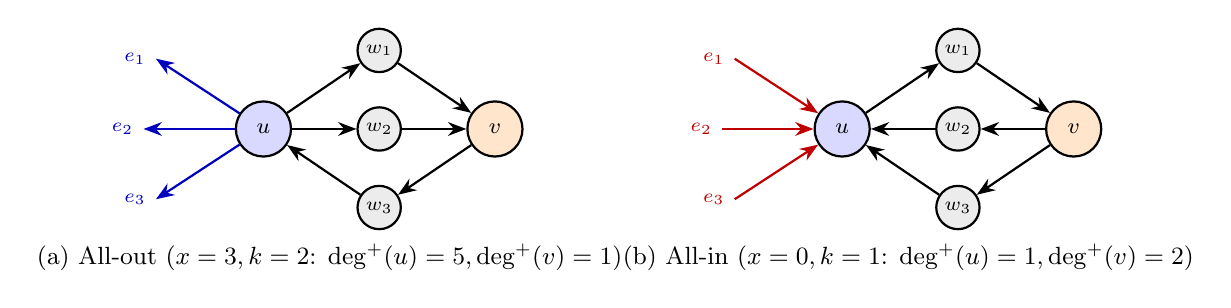
\begin{tikzpicture}[scale=1.05,
  >=Stealth,
  v6/.style={circle,draw,fill=blue!15,thick,minimum size=7mm,inner sep=1pt,font=\footnotesize},
  v3/.style={circle,draw,fill=orange!20,thick,minimum size=7mm,inner sep=1pt,font=\footnotesize},
  v2/.style={circle,draw,fill=gray!15,thick,minimum size=5.5mm,inner sep=1pt,font=\scriptsize}]

  % Left: all-out state (x=3, k=2)
  \begin{scope}[shift={(-3.5,0)}]
    \node[v6] (u) at (0,0) {$u$};
    \node[v3] (v) at (2.8,0) {$v$};
    \node[v2] (w1) at (1.4,0.95) {$w_1$};
    \node[v2] (w2) at (1.4,0) {$w_2$};
    \node[v2] (w3) at (1.4,-0.95) {$w_3$};

    \draw[thick,->,blue!75!black] (u) -- (-1.3, 0.85) node[left,font=\scriptsize] {$e_1$};
    \draw[thick,->,blue!75!black] (u) -- (-1.45, 0) node[left,font=\scriptsize] {$e_2$};
    \draw[thick,->,blue!75!black] (u) -- (-1.3, -0.85) node[left,font=\scriptsize] {$e_3$};

    \draw[thick,->] (u) -- (w1); \draw[thick,->] (w1) -- (v);
    \draw[thick,->] (u) -- (w2); \draw[thick,->] (w2) -- (v);
    \draw[thick,->] (v) -- (w3); \draw[thick,->] (w3) -- (u);

    \node[font=\small] at (0.8,-1.55) {(a) All-out ($x=3, k=2$: $\outdeg(u)=5, \outdeg(v)=1$)};
  \end{scope}

  % Right: all-in state (x=0, k=1)
  \begin{scope}[shift={(3.5,0)}]
    \node[v6] (u) at (0,0) {$u$};
    \node[v3] (v) at (2.8,0) {$v$};
    \node[v2] (w1) at (1.4,0.95) {$w_1$};
    \node[v2] (w2) at (1.4,0) {$w_2$};
    \node[v2] (w3) at (1.4,-0.95) {$w_3$};

    \draw[thick,<-,red!75!black] (u) -- (-1.3, 0.85) node[left,font=\scriptsize] {$e_1$};
    \draw[thick,<-,red!75!black] (u) -- (-1.45, 0) node[left,font=\scriptsize] {$e_2$};
    \draw[thick,<-,red!75!black] (u) -- (-1.3, -0.85) node[left,font=\scriptsize] {$e_3$};

    \draw[thick,->] (u) -- (w1); \draw[thick,->] (w1) -- (v);
    \draw[thick,->] (v) -- (w2); \draw[thick,->] (w2) -- (u);
    \draw[thick,->] (v) -- (w3); \draw[thick,->] (w3) -- (u);

    \node[font=\small] at (0.8,-1.55) {(b) All-in ($x=0, k=1$: $\outdeg(u)=1, \outdeg(v)=2$)};
  \end{scope}
\end{tikzpicture}
\caption{The $5$-vertex equality splitter gadget $S_3$ ($\deg(u)=6, \deg(v)=3, \deg(w_i)=2$) and its two admissible external states: all three external half-edges $(e_1, e_2, e_3)$ must agree.}
\label{fig:splitter}
\end{figure}

\begin{theorem}[NP-completeness at $\Delta(G) = 6$]\label{thm:npc}
Deciding whether a simple bipartite graph $G$ with $\Delta(G) = 6$ (and all vertex degrees in $\{2, 3, 6\}$) admits a coprime orientation is \textbf{NP}-complete.
\end{theorem}

\begin{proof}
Membership in \textbf{NP} is immediate: an orientation $D$ is a polynomial-size certificate, and verifying $\gcd(\outdeg_D(v), \indeg_D(v)) = 1$ for all $v \in V$ takes polynomial time.

For \textbf{NP}-hardness, we reduce from \textsc{Monotone NAE-3SAT}~\cite{Schaefer1978}: given a set of Boolean variables $X = \{x_1, \dots, x_n\}$ and a collection of $3$-element clauses $\mathcal{C} = \{C_1, \dots, C_m\}$ (each $C_j = \{x_{j,1}, x_{j,2}, x_{j,3}\}$ with three distinct variables), decide whether there exists a truth assignment $\tau : X \to \{\mathsf{T}, \mathsf{F}\}$ such that every clause contains at least one $\mathsf{T}$ and at least one $\mathsf{F}$.

Given an instance $(X, \mathcal{C})$ of \textsc{Monotone NAE-3SAT}, we construct a graph $G$ as follows:
\begin{enumerate}[leftmargin=2em,itemsep=2pt]
  \item \emph{Duplicated clause vertices:} Create two disjoint copies $\mathcal{C}^{(1)}$ and $\mathcal{C}^{(2)}$ of the clause set $\mathcal{C}$. For each clause $C_j \in \mathcal{C}$, introduce two degree-$3$ vertices $c_j^{(1)}$ and $c_j^{(2)}$, one for each copy.
  \item \emph{Variable gadgets:} Discard any variable that appears in no clause. For each variable $x_i$ appearing $r_i \ge 1$ times in $\mathcal{C}$, take a cycle of $2 r_i$ copies of the equality splitter gadget $S_3$ with degree-$6$ centers $u_i^{(0)}, u_i^{(1)}, \dots, u_i^{(2r_i - 1)}$: for each $s \in \{0, \dots, 2r_i - 1\}$, identify one external port of $u_i^{(s)}$ with one external port of $u_i^{(s+1 \bmod 2r_i)}$ by a connecting edge (note that for $r_i = 1$, this places two parallel edges between $u_i^{(0)}$ and $u_i^{(1)}$, which become internally disjoint length-$2$ paths in Step~3). Each center $u_i^{(s)}$ now has exactly one remaining free external port. Connect the $r_i$ free ports of the \emph{positive} centers $u_i^{(2t)}$ ($0 \le t < r_i$) to the $r_i$ clause vertices in $\mathcal{C}^{(1)}$ containing $x_i$, and connect the $r_i$ free ports of the \emph{negative} centers $u_i^{(2t+1)}$ ($0 \le t < r_i$) to the $r_i$ clause vertices in $\mathcal{C}^{(2)}$ containing $x_i$.
  \item \emph{Bipartization and simplification:} Subdivide every edge of $G$ once with a degree-$2$ vertex to obtain a graph $G'$. By Proposition~\ref{prop:subdiv}, $G'$ is simple, bipartite, has polynomial size $O(n + m)$, has all vertex degrees in $\{2, 3, 6\}$, and is coprimely orientable if and only if $G$ is coprimely orientable.
\end{enumerate}

Let us verify correctness. In any coprime orientation $D$ of $G$, Lemma~\ref{lem:splitter} forces every splitter center $u_i^{(s)}$ to have all three of its external edges either all directed out of $u_i^{(s)}$ (call this state $\mathsf{T}$) or all directed into $u_i^{(s)}$ (call this state $\mathsf{F}$). Because $u_i^{(s)}$ and $u_i^{(s+1 \bmod 2r_i)}$ share an external edge, their states must be \emph{opposite}: all positive centers $u_i^{(2t)}$ share a common state $\tau(x_i) \in \{\mathsf{T}, \mathsf{F}\}$, and all negative centers $u_i^{(2t+1)}$ share the negated state $\neg \tau(x_i)$.

Consequently:
\begin{itemize}[leftmargin=2em,itemsep=1pt]
  \item Every clause vertex $c_j^{(1)}$ in $\mathcal{C}^{(1)}$ receives incoming arcs from precisely those $x_i \in C_j$ with $\tau(x_i) = \mathsf{T}$, and sends outgoing arcs to those with $\tau(x_i) = \mathsf{F}$. Since $\deg_G(c_j^{(1)}) = 3$, $\outdeg_D(c_j^{(1)}) \in \Aset(3) = \{1, 2\}$ holds if and only if $C_j$ is NAE-satisfied by $\tau$.
  \item Every clause vertex $c_j^{(2)}$ in $\mathcal{C}^{(2)}$ sees the negated assignment $\neg \tau$, which NAE-satisfies $C_j$ if and only if $\tau$ NAE-satisfies $C_j$ (since NAE is invariant under global negation!).
\end{itemize}
Conversely, any NAE-satisfying assignment $\tau$ of $(X, \mathcal{C})$ sets each positive center $u_i^{(2t)}$ to state $\tau(x_i)$ and each negative center $u_i^{(2t+1)}$ to $\neg \tau(x_i)$, which extends by Lemma~\ref{lem:splitter} to a valid coprime orientation of $G$.
\end{proof}

% ============================================================================
\section{Machine-Checked Formal Verification in Lean~4}
% ============================================================================

To ensure complete mathematical rigor, we formalized the core arithmetic, structural, classification, obstruction, and gadget theorems of this paper in \texttt{Lean~4} (v4.36.0) in the standalone module \texttt{CoprimeOrientations.lean}. The formalization uses zero external libraries (pure Lean~4 core), zero custom axioms, and zero \texttt{sorry}s, and compiles in under $20$ seconds via \texttt{lake build}. Table~\ref{tab:lean} summarizes the correspondence between paper results and machine-checked Lean~4 theorems.

\begin{table}[ht]
\centering
\small
\begin{tabular}{@{}lll@{}}
\toprule
\textbf{Paper Result} & \textbf{Lean~4 Theorem Name} & \textbf{Scope} \\
\midrule
Prop.~\ref{prop:basic}(i)--(iii) & \texttt{isCoprimeOut\_iff\_gcd\_deg}, \texttt{isCoprimeOut\_rev} & All $d, k \in \N$ \\
Thm.~\ref{thm:odd} (arith.) & \texttt{coprime\_balanced\_odd} & All $m \in \N$ \\
Thm.~\ref{thm:pow2} (arith.) & \texttt{isCoprimeOut\_pow\_two} & All $m \ge 1, k \in \N$ \\
Thm.~\ref{thm:bipartite}(b) & \texttt{complete\_bipartite\_coprime} & All $a, b \ge 1$ \\
Thm.~\ref{thm:Kn} & \texttt{complete\_graph\_coprime\_iff} & All $n \ge 1$ \\
Thm.~\ref{thm:eulerian} & \texttt{eulerian\_parity\_obstruction} & All finite graphs \\
Thm.~\ref{thm:mod4}(a) & \texttt{six\_all\_mod4\_eq\_one}, \texttt{even\_ne\_six\_has\_diff\_two} & All even $d \ge 4$ \\
Thm.~\ref{thm:mod4}(b) & \texttt{six\_regular\_cut\_obstruction} & All odd $s$, cut $\in \{0,2\}$ \\
Thm.~\ref{thm:gap} & \texttt{prime\_power\_gap\_dichotomy} & All $d \ge 1$ \\
Lem.~\ref{lem:splitter} & \texttt{splitter\_gadget\_iff} & All $e_1, e_2, e_3 \in \mathsf{Bool}$ \\
\bottomrule
\end{tabular}
\caption{Correspondence between paper theorems and machine-checked proofs in \texttt{CoprimeOrientations.lean}.}
\label{tab:lean}
\end{table}

% ============================================================================
\section{Open Problems}
% ============================================================================

We conclude with four natural open problems suggested by our results.

\begin{problem}[Regular NP-completeness]
Is \textsc{Coprime Orientation} \textbf{NP}-complete when restricted to $6$-regular graphs (without degree-$2$ or degree-$3$ vertices)?
\end{problem}

\begin{problem}[Planar graphs]
Is \textsc{Coprime Orientation} \textbf{NP}-complete for planar graphs with $\Delta(G) \le 6$? Note that our reduction uses \textsc{Monotone NAE-3SAT}, whose planar restriction is in \textbf{P}~\cite{Moret1988}; a planar hardness proof would likely require a reduction from \textsc{Planar 3-SAT} or \textsc{Planar 1-in-3 SAT} using a global polarity gadget.
\end{problem}

\begin{problem}[Characterization of coprimely orientable $6$-regular graphs]
By Theorem~\ref{thm:mod4}(b), a $6$-regular graph with an odd-sized vertex cut of size $0$ or $2$ is not coprimely orientable. Does every $4$-edge-connected $6$-regular graph on an even number of vertices admit a coprime orientation?
\end{problem}

\begin{problem}[Enumeration and random graphs]
What is the asymptotic behavior of $\cop(G)$ for $d$-regular graphs and Erd\H{o}s--R\'enyi random graphs $G(n, p)$? In particular, what is the threshold probability $p(n)$ at which $G(n, p)$ is asymptotically almost surely coprimely orientable?
\end{problem}

\begin{thebibliography}{10}

\bibitem{AlonTarsi1992}
N.~Alon and M.~Tarsi,
\emph{Colorings and orientations of graphs},
Combinatorica \textbf{12} (1992), 125--134.

\bibitem{Chevalier1983}
O.~Chevalier, F.~Jaeger, C.~Payan, and N.~H.~Xuong,
\emph{Odd rooted orientations and upper-embeddable graphs},
Annals of Discrete Mathematics \textbf{17} (1983), 177--181.

\bibitem{Cornuejols1988}
G.~Cornu\'ejols,
\emph{General factors of graphs},
Journal of Combinatorial Theory, Series B \textbf{45} (1988), 185--198.

\bibitem{Frank1980}
A.~Frank,
\emph{On the orientation of graphs},
Journal of Combinatorial Theory, Series B \textbf{28} (1980), 251--261.

\bibitem{Hakimi1965}
S.~L.~Hakimi,
\emph{On the degrees of the vertices of a directed graph},
Journal of the Franklin Institute \textbf{279} (1965), 290--308.

\bibitem{ListAvoiding2024}
J.~A.~Akhlaghi, B.~Mohar, and M.~Rostami,
\emph{List-avoiding orientations},
preprint / NSF PAR 10597046 (2024).

\bibitem{Moret1988}
B.~M.~E.~Moret,
\emph{Planar NAE3SAT is in P},
ACM SIGACT News \textbf{19} (1988), 51--54.

\bibitem{Robbins1939}
H.~E.~Robbins,
\emph{A theorem on graphs, with an application to a problem of traffic control},
American Mathematical Monthly \textbf{46} (1939), 281--283.

\bibitem{Schaefer1978}
T.~J.~Schaefer,
\emph{The complexity of satisfiability problems},
Proceedings of the 10th Annual ACM Symposium on Theory of Computing (STOC 1978), 216--226.

\end{thebibliography}

\end{document}
